%%%%%%%%%%%%%%%%%%%%%%%%%%%%%%%%%%%%%%%%
%% MCM/ICM LaTeX Template %%
%% 2026 MCM/ICM           %%
%%%%%%%%%%%%%%%%%%%%%%%%%%%%%%%%%%%%%%%%
\documentclass[12pt]{article}
\usepackage{geometry}
\geometry{left=1in,right=0.75in,top=1in,bottom=1in}

%%%%%%%%%%%%%%%%%%%%%%%%%%%%%%%%%%%%%%%%
% Replace ABCDEF in the next line with your chosen problem
% and replace 1111111 with your Team Control Number
\newcommand{\Problem}{B}
\newcommand{\Team}{2629090}
%%%%%%%%%%%%%%%%%%%%%%%%%%%%%%%%%%%%%%%%

\usepackage{newtxtext}
\usepackage{amsmath,amssymb,amsthm}
\usepackage{newtxmath} % must come after amsXXX

\usepackage[pdftex]{graphicx}
\usepackage{xcolor}
\usepackage{fancyhdr}
\usepackage{longtable}
\lhead{Team \Team}
\rhead{}
\cfoot{}

\newtheorem{theorem}{Theorem}
\newtheorem{corollary}[theorem]{Corollary}
\newtheorem{lemma}[theorem]{Lemma}
\newtheorem{definition}{Definition}

%%%%%%%%%%%%%%%%%%%%%%%%%%%%%%%%
\begin{document}
\graphicspath{{.}}  % Place your graphic files in the same directory as your main document
\DeclareGraphicsExtensions{.pdf, .jpg, .tif, .png}
\thispagestyle{empty}
\vspace*{-16ex}
\centerline{\begin{tabular}{*3{c}}
	\parbox[t]{0.3\linewidth}{\begin{center}\textbf{Problem Chosen}\\ \Large \textcolor{red}{\Problem}\end{center}}
	& \parbox[t]{0.3\linewidth}{\begin{center}\textbf{2026\\ MCM/ICM\\ Summary Sheet}\end{center}}
	& \parbox[t]{0.3\linewidth}{\begin{center}\textbf{Team Control Number}\\ \Large \textcolor{red}{\Team}\end{center}}	\\
	\hline
\end{tabular}}
%%%%%%%%%%% Begin Summary %%%%%%%%%%%
% Enter your summary here replacing the (red) text
% Replace the text from here ...
\begin{center}

With the increasing demands for lunar base construction and long-term operation, the Earth-Moon transportation system faces systemic constraints in terms of efficiency, cost, and environmental impact. This modeling team focuses on material transportation during the lunar base construction phase, constructing a multi-channel transportation modeling framework that comprehensively considers time, cost, and environmental pollution. The aim is to evaluate the feasibility and optimal configuration of rockets and space elevators under different conditions and provide quantitative basis for long-term engineering planning.

Regarding the first problem, this paper establishes throughput models for rocket transportation channels and space elevator channels under ideal operating conditions, characterizing their annual effective transportation capacity and cost structure. Based on this, the Pareto method is used to analyze the completion time and cost characteristics of single transportation modes and combined transportation schemes under a given total construction mass, and to preliminarily compare the differences in time and cost dimensions among different transportation structures.

Regarding the second problem, adverse factors such as weather fluctuations and operational accidents are further introduced to correct for rocket transportation efficiency and cost, and a stochastic process is used to describe interannual operational uncertainty. Monte Carlo simulation is used to evaluate the distribution characteristics of the system's effective throughput capacity under suboptimal conditions, obtaining the time-cost evolution trend of the combined transportation system in an unstable environment, thereby characterizing the system's robustness and risk range.

To address problem three, and to better reflect potential operational scenarios, this paper introduces a water cycle and storage mechanism, transforming the demand for building materials into the need to maintain a minimum water supply. Under the influence of factors from problem two, Monte Carlo simulations are used to analyze the risk of water shortage in the combined transport system's allocation ratio and the confidence interval for the base's water storage capacity over 10 years. This, combined with cost considerations, identifies the safest and most cost-effective transport solution.

For problem four, building upon the model from problem two, this paper introduces environmental impact indicators, constructing a comprehensive evaluation index vector centered on time, cost, and carbon emissions. Using the Pareto method, the paper systematically compares the non-dominated solution sets of different transport configurations under multi-objective constraints, revealing the trade-off between the rocket transport ratio and the size of the space elevator on overall efficiency and environmental costs, and identifying engineering-significant compromise solutions.

This paper includes data visualization and error analysis after each problem. The results show that the proposed combined transport modeling framework maintains consistent trend judgments under different assumptions, exhibits good structural stability, and can provide effective quantitative support for future planning and decision-making in the Earth-Moon transport system. Considering the complexity of mechanisms in reality, this paper adopts the ideas of isomorphism and systems engineering in modeling, so that the model of each question is a variation of the basic model, while the influencing factors can be modeled separately and entered into the basic model in a unified form, ensuring that the model still has the convenience and credibility of modification and factor introduction under real conditions.

\end{center}
% to here
%%%%%%%%%%% End Summary %%%%%%%%%%%

%%%%%%%%%%%%%%%%%%%%%%%%%%%%%%
\clearpage
\pagestyle{fancy}
% Uncomment the next line to generate a Table of Contents
\tableofcontents
\newpage
\setcounter{page}{1}
\rhead{Page \thepage\ }
%%%%%%%%%%%%%%%%%%%%%%%%%%%%%%
\section{Introduction}

\subsection{Problem Background}

With the development of deep space exploration technology, human exploration of the moon is gradually shifting from short-term missions to long-term stays and large-scale construction. Against this backdrop, the transportation of large quantities of supplies between Earth and the moon has become a key factor restricting the progress and cost of lunar base construction. The construction of lunar base infrastructure requires a continuous, stable, and high-throughput supply of materials, but existing single transportation methods have significant limitations in terms of efficiency, economy, and environmental impact.

Traditional rocket transportation has advantages such as mature technology and flexible deployment, but its unit transportation cost is high, it is significantly affected by weather and launch conditions, and it is accompanied by high energy consumption and carbon emissions. In contrast, space elevators, as a potential continuous transportation method, can theoretically provide stable and low-energy transportation capabilities in long-term operation, but their construction cycle is long, initial investment is huge, and there are significant constraints in system scale and operational phases. Therefore, how to rationally allocate different transportation methods in a practical engineering context to form a complementary and synergistic joint transportation system is a system optimization problem of practical significance.

From an engineering planning perspective, the construction of a lunar base is not a one-time completion, but a dynamic process that spans many years and progresses gradually. Transportation systems not only need to meet overall construction goals, but also need to balance the relationship between completion time, economic costs, and environmental impact at different stages. This makes it difficult for optimal solutions based on a single indicator to meet actual needs, necessitating a systemic analysis and evaluation of the transportation system within a multi-objective framework.

\subsection{Restatement of the Problem}

Considering the background information and restrictedconditions identified in the problem statement, we need tosolve the following problems:

Problem 1:Consider the time, cost, and transportation strategy for three transportation scenarios under ideal operating conditions.

Problem 2:Considering time, cost, and transportation strategies that include undesirable factors.

Problem 3:Propose a transportation strategy that considers both safety and cost under sustained demand.

Problem 4:Taking environmental impact into account, a comprehensive assessment of time and cost is proposed.

\subsection{Our Work}

This paper constructs a unified quantitative framework for evaluating large-scale orbital transportation systems under various practical constraints. It focuses on the complementary application of conventional rockets and space elevators, and the work is divided into four main phases.

First, we establish a baseline transportation model describing the nominal throughput, time, and cost structure of each transportation channel. Rocket systems are characterized by discrete launch phases and batch constraints, while space elevators are modeled as continuous flow channels with a fixed annual capacity. This provides a unified reference point for subsequent analyses.

Second, we incorporate adverse and uncertain factors into the system. Weather conditions and accident risks are introduced through multiplicative efficiency and cost correction factors, allowing stochastic external disturbances to be directly reflected in effective capacity and unit cost. Furthermore, we quantify environmental impact by defining carbon emission intensity per unit transport mass, thus incorporating sustainability factors into the assessment.

Third, based on the above model, we construct a multi-objective optimization problem with transport time, total cost, and environmental impact as core indicators. Through scenario analysis of different channel combinations and parameter settings, we generate a Pareto front, clearly revealing the trade-offs between efficiency, economy, and sustainability. This analysis highlights the applicable scenarios where hybrid transport strategies outperform single-lane solutions.

Finally, we use representative parameter values for numerical simulations to validate the analysis results. The simulation results demonstrate the robustness of the proposed framework and show how decision-makers can find balanced solutions under real-world operational constraints.

In summary, our work provides a structured and scalable approach to evaluating complex rail transit systems, integrating physical modeling, risk adjustment, and multi-objective decision analysis into a unified framework.

\begin{figure}[htbp]
    \centering
    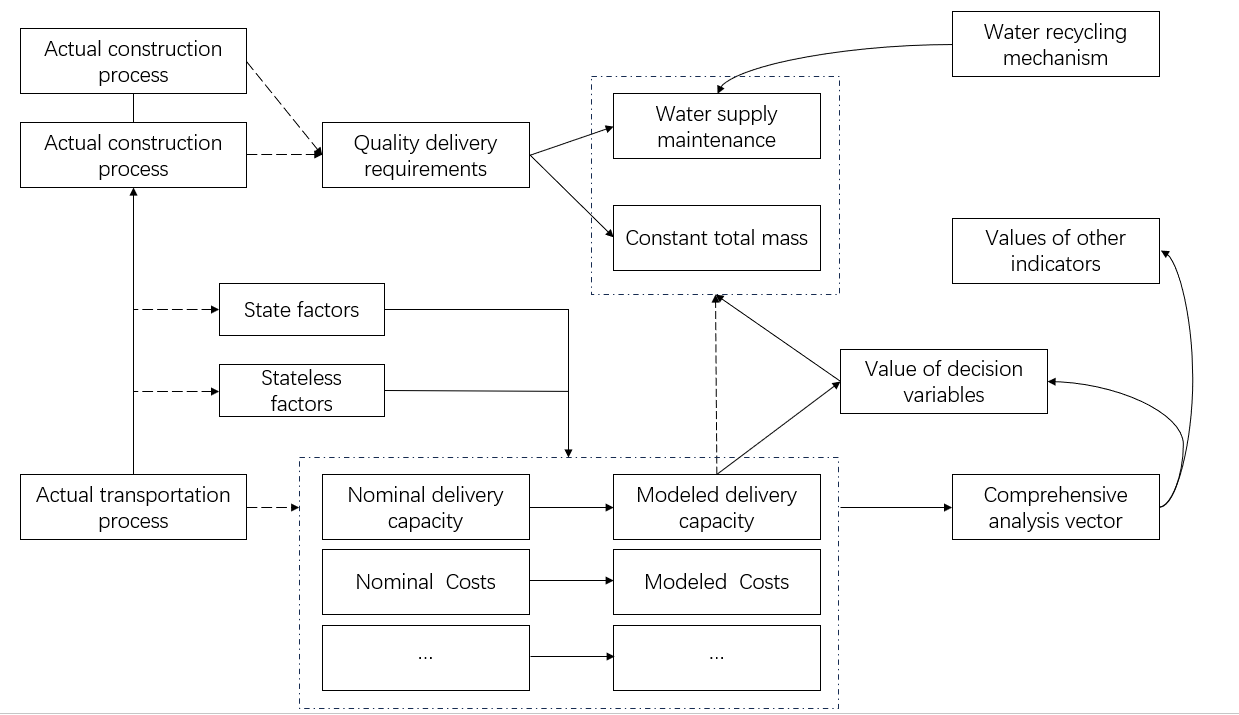
\includegraphics[width=0.8\linewidth]{fig0.png}
    \caption{Basic concept diagram of the model}
    \label{fig:fig0}
\end{figure}

\section{Assumptions and Justifications}

Considering that the total amount of transported materials required for the construction of a lunar colony is approximately $10^8$ tons, preliminary estimates suggest that the overall construction cycle will be on the order of a century. Explicitly characterizing the transportation process at the lunar or even daily scale in the model would not only significantly increase model complexity but also make it difficult to obtain stable and interpretable results within a limited timeframe. Furthermore, even under idealized transportation conditions, the annual scale is inevitably affected by periodic constraints such as the Earth-Moon phase. Some of these factors directly impact the transportation process, while others reduce overall transportation efficiency. Therefore, based on the matching of problem size and planning objectives, this paper selects "year" as the sole explicit time scale to characterize core indicators such as delivery volume and cost. Factors directly related to the transportation process are incorporated into the construction of annual nominal indicators, while other less-than-ideal factors, after precise modeling, are uniformly transformed into annual-scale efficiency reduction coefficients. Through this approach, the model maintains continuity in the time dimension while avoiding the sacrifice of accuracy in characterizing key influencing factors due to the time scale.

\subsection{Model Assumptions}
\subsubsection{Time model}
Let $t \in \mathbb{R}$ denote time. The time interval $\Delta t$ is defined as
\[
\Delta t = t_1 - t_0 .
\]
At the initiation of the project, the time origin is defined as $t_{\text{begin}} = 0$.

\subsubsection{Continuous-time cumulative model of throughput at transportation nodes}
Let $q_i(\Phi_i)$ denote the throughput of the $i$-th transportation node per unit time, and let $Q_i(t)$ denote the cumulative total throughput of the $i$-th transportation node from the initiation of the project up to time $t$. Then,
\[
Q_i(t_1) - Q_i(t_0) = \int_{t_0}^{t_1} q_i(\Phi_i)\, dt .
\]

Here, $\Phi_i$ represents the set of factors that influence the per-unit-time throughput of the transportation node, where each factor is modeled by one or more variables.

In real-world transportation systems, the throughput per unit time is bounded, that is,
\[
q_i \le q^{\text{nominal}} .
\]

For convenience of computation, the unit of $q$ is defined as metric tons.

\subsubsection{Cumulative Quality Model of Project Delivery}
The construction of a lunar colony can be regarded as a process characterized by a total mass requirement $M_{\text{total}}$ and a total completion time $t_{\text{total}}$, where
\[
M_{\text{total}} = 10^8 + M_{\text{others}} ,
\]
\[
t_{\text{total}} = t_{\text{trans}} + t_{\text{build}} .
\]

Under ideal conditions, the total mass requirement consists solely of construction materials, and the total completion time $t_{\text{total}}$ is entirely determined by the total transportation time $t_{\text{trans}}$, which includes both transportation preparation time and in-transit time. In this idealized setting, no temporal coordination between construction and transportation is considered. Consequently, the completion time of the project is determined only by whether the cumulative delivered mass reaches the required demand.

Let $\mu$ denote the mass ratio between construction materials and other payloads. The delivered mass per unit time $m_i$ and the cumulative delivered mass $M_i$ are defined as
\[
m_i = \mu q_i ,
\]
\[
M_i(t_1) - M_i(t_0) = \int_{t_0}^{t_1} m_i(\Phi_i)\, dt .
\]

Accordingly, the completion condition of the construction under the context of this problem is given by
\[
\sum_i M_i(t_{\text{end}}) \ge M_{\text{total}} ,
\]
where $t_{\text{end}}$ denotes the time at which the project is completed.

\subsection{Decision variable modeling}

Let $\sigma \in [0,1]$ denote the mass allocation ratio assigned to rocket-based transportation. Then,
\[
M_{\text{total}}^{TR} = \sigma M_{\text{total}} , \quad M_{\text{total}}^{SE} = (1 - \sigma) M_{\text{total}} .
\]

Furthermore, both methods that activate only the rocket and methods that activate only the space elevator can be given by the value of sigma.

\subsection{Multi-indicator cumulative evaluation model}

\subsubsection{Cost model}
Let $C_i(t)$ denote the cumulative total cost incurred by transportation node $i$ from the start of construction up to time $t$, and let $c_i(\Lambda_i)$ denote the cost incurred per unit time. Then,
\[
C_i(t_1) - C_i(t_0) = \int_{t_0}^{t_1} c_i(\Lambda_i)\, dt .
\]

Here, $\Lambda_i$ represents the set of factors that influence the per-unit-time cost of the transportation node, where each factor is modeled by one or more variables.

For convenience of computation, the unit of cost is defined as hundreds of millions of U.S. dollars.

\subsubsection{Negative effect cumulative model}
Let $E_i(t)$ denote the cumulative total negative impact (e.g., environmental pollution) generated by transportation node $i$ from the start of construction up to time $t$, and let $e_i(\Psi_i)$ denote the negative impact incurred per unit time. Then,
\[
E_i(t_1) - E_i(t_0) = \int_{t_0}^{t_1} e_i(\Psi_i)\, dt .
\]

Here, $\Psi_i$ represents the set of factors that influence the per-unit-time negative impact of the transportation node, where each factor is modeled by one or more variables.

This indicator is used to comprehensively characterize the negative impacts on the environment or the system during transportation, and its value is e

\subsubsection{Comprehensive indicators}
Define the comprehensive evaluation indicator vector as
\[
\boldsymbol{K} = ( T, C, E, \ldots )^\top ,
\]
where
\[
T = t_{\text{end}} - t_{\text{begin}} .
\]

In this context, the only difference between the different options lies in the ratio of the transport mission mass allocated to the rocket launch site and the space elevator. Therefore

\[
\boldsymbol{K(\sigma)} = \{ T(\sigma), C(\sigma), E(\sigma), \ldots \} ,
\]

Let $\boldsymbol{a},\boldsymbol{b}\in\mathbb{R}^n$.
The notation $\boldsymbol{a}\preceq\boldsymbol{b}$ denotes
componentwise inequality, i.e.,
$a_i\le b_i$ for all components.

For two feasible schemes $\sigma_1,\sigma_2\in\mathcal S$,
$\sigma_1$ is said to Pareto dominate $\sigma_2$ if
\[
\boldsymbol K(\sigma_1)\preceq \boldsymbol K(\sigma_2),
\quad
\boldsymbol K(\sigma_1)\ne \boldsymbol K(\sigma_2).
\]

A scheme $\sigma^\ast\in\mathcal S$ is Pareto optimal if there exists no
$\sigma\in\mathcal S$ such that
\[
\boldsymbol K(\sigma)\preceq \boldsymbol K(\sigma^\ast),
\quad
\boldsymbol K(\sigma)\ne \boldsymbol K(\sigma^\ast).
\]

The Pareto frontier is defined as
\[
\mathcal P
=
\left\{
\sigma\in\mathcal S \,\middle|\,
\nexists\,\sigma'\in\mathcal S :
\boldsymbol K(\sigma')\preceq \boldsymbol K(\sigma),
\;
\boldsymbol K(\sigma')\ne \boldsymbol K(\sigma)
\right\}.
\]


\subsection{State-based modeling mechanism of influencing factors}

When modeling influencing factors with monthly or even daily scale characteristics, we categorize them into two types. One type of factor only affects the annual transportation efficiency of the current year, and its impact does not accumulate across years; the other type of factor exhibits a clear state-dependent characteristic, meaning that its impact in the current year will have a lasting effect on transportation conditions in the following year. Based on this difference, this paper uses different parameterization methods to characterize the two types of factors.

Under this mechanism, the set of factors influencing the throughput capacity of a transportation node, denoted by $\Phi$, is divided into two categories: stateless factors $\boldsymbol{\alpha}$ and state-dependent factors $\boldsymbol{\beta}(t)$. Stateless factors describe efficiency or availability differences that can be regarded as constant over the study time scale, while state-dependent factors describe system states that are inherited from year to year. The evolution of the state-dependent factors satisfies
\[
\boldsymbol{\beta}(t+1) = F(\boldsymbol{\beta}(t), \text{others}) .
\]

Furthermore, considering that some operational states occur only within a single year and are reset at the end of the year, such as short-term scheduling fluctuations or single-launch anomalies, only state variables with inter-annual inheritance effects are included in $\boldsymbol{\beta}(t)$. Intra-annual states are equivalently incorporated into the stateless factors $\boldsymbol{\alpha}$ through process-level analysis or statistical expectation.

Let $A(\boldsymbol{\alpha}_i) \in [0,1]$ and $B(\boldsymbol{\beta}_i(t)) \in [0,1]$ denote the comprehensive efficiency coefficients corresponding to stateless and state-dependent factors, respectively. Then, the actual throughput per unit time of a transportation node under realistic operating conditions can be expressed as
\[
q_i(\Phi_i) = A(\boldsymbol{\alpha}_i)\, B(\boldsymbol{\beta}_i(t))\, q_i^{\text{nominal}} .
\]

Under fully ideal conditions, $A = B = 1$.

In this formulation, each individual influencing factor $\alpha_{i,k}$ or $\beta_{i,k}$ is treated as a degradation coefficient of the per-unit-time throughput capacity, with values in the range $[0,1]$. The comprehensive efficiency functions $A$ and $B$ adopt a multiplicative combination of these degradation coefficients. This structure allows weakly correlated factors to be modeled independently, while strongly correlated factors can be handled by merging them into a single composite factor, achieving a balance between modeling independence and real-world correlation. Similar state-based modeling methods can be directly extended to the cost factor set $\Lambda$ and the adverse impact factor set $\Psi$, ensuring that different evaluation indicators share a consistent structural form under a unified state description.

It should be noted that this paper's definition of "stateness" remains strictly based on the annual scale. If a factor's state change on a monthly scale affects subsequent months, but its annual average state does not affect the following year, then this factor should be included in the efficiency coefficient $\alpha$ through its statistical mean or expected value, rather than being considered a state variable $\beta$. This principle ensures the model's consistency on the annual scale while avoiding misjudging high-frequency fluctuations as long-term structural effects.

\subsection{Parameterization of Nominal Transportation Capacity and Cost}

In the context of this question, $M_{total}=1\times 10^8$

In the problem statement, the transport capacity of the space elevator is given in the form of annual throughput, while the rocket transport capacity is represented by the payload per launch. To compare and integrate the two transport methods on a unified timescale, it is necessary to convert the rocket's discrete launch capacity into a nominal transport capacity on an annual scale. This process requires comprehensively considering factors such as the Earth-Moon phase that constrain the launch window, thereby obtaining the rocket's equivalent nominal transport capacity on an annual scale.

For the $i$-th rocket transportation node, the nominal annual throughput is defined as
\[
q_{i,\mathrm{nominal}}^{\mathrm{TR}}
= N_{\mathrm{phase}} \cdot D_{\mathrm{phase}} \cdot N_{\mathrm{launch}} \cdot m_{\mathrm{rocket}},
\]
where $N_{\mathrm{phase}}$ denotes the number of available launch phases within one year, $D_{\mathrm{phase}}$ represents the duration in days of each launch phase, $N_{\mathrm{launch}}$ is the maximum number of launches that a single launch site can perform per day, and $m_{\mathrm{rocket}}$ is the nominal effective payload mass of a single rocket.

In the context of this question, we can assume that $m_{rocket} = 150$, $i^{TR}=1,2, \cdots,10$

It is worth noting that the above factors should not be included in the efficiency coefficient $\alpha$ or the state coefficient $\beta$, because they are not a reduction of a given transport capacity, but rather preconditions constituting the basic assumptions of the annual nominal transport capacity. This distinction helps maintain the clarity of the model structure and avoids confusion regarding the parameter meanings of factors at different levels.

Correspondingly, the average annual cost per unit time of the $i$-th rocket transportation node is defined as
\[
c_i^{\mathrm{TR}}(\Lambda_i)
= C_{\mathrm{prep}} + N_{\mathrm{phase}} \cdot D_{\mathrm{phase}} \cdot N_{\mathrm{launch}} \cdot c_{\mathrm{launch}},
\]
where $C_{\mathrm{prep}}$ denotes the fixed preparation cost required for a single annual launch campaign, and $c_{\mathrm{launch}}$ represents the equivalent cost per launch of a single rocket under long-term reusable operation, which already accounts for the initial manufacturing cost and the allowable number of reuse cycles.

For the $i$-th space elevator transportation node, the nominal annual throughput is directly determined by the system design capacity and is given by
\[
q_{i,\mathrm{nominal}}^{\mathrm{SE}} = Q_{\mathrm{SE}} = 1.7 \times 10^{5}.
\]
And $i^{SE}=1,2,3$
The average annual cost per unit time of the space elevator node is defined as
\[
c_i^{\mathrm{SE}}(\Lambda_i)
= C_{\mathrm{SE,day}} \cdot D_{\mathrm{year}},
\]
where $C_{\mathrm{SE,day}}$ denotes the average daily operating cost of the space elevator, including capsule preparation, propulsion, and system maintenance, and $D_{\mathrm{year}}$ represents the number of calendar days in one year.

By the way,for reusable rockets, the per-launch cost is treated in an equivalent averaged form. Specifically,
\[
c_{\mathrm{launch}}
= \frac{C_{\mathrm{init}} + N_{\mathrm{reuse}} \cdot C_{\mathrm{reuse}}}{N_{\mathrm{reuse}}}.
\]
This formulation evenly distributes the one-time manufacturing cost over all allowable reuse cycles, thereby rendering each launch economically equivalent under long-term, steady-state operation.

If individual rocket failures or reliability degradation are explicitly considered, additional state variables must be introduced to describe the launch status. However, the resulting modeling framework remains structurally isomorphic to the throughput formulation and can be incorporated in a consistent manner.

\section{Variables and Notations}

\begin{longtable}{p{3.8cm} p{10.2cm}}
\caption{Core Model Variables and Notations} \\
\hline
\textbf{Variable} & \textbf{Description} \\
\hline
\endfirsthead

\hline
\textbf{Variable} & \textbf{Description} \\
\hline
\endhead

\hline
\endfoot

\hline
\endlastfoot

$t$ & Continuous time variable \\

$t_{\text{begin}}$ & Project start time, defined as zero \\
$t_{\text{end}}$ & Project completion time \\
$T$ & Total construction period, $T = t_{\text{end}} - t_{\text{begin}}$ \\

$q_i(\boldsymbol{\Phi}_i)$ & Effective throughput per unit time of transportation node $i$ under influencing factors $\boldsymbol{\Phi}_i$ \\
$Q_i^{\text{nominal}}$ & Nominal (ideal) throughput capacity of transportation node $i$ \\
$Q_i(t)$ & Cumulative delivered throughput of transportation node $i$ up to time $t$ \\

$M_{\text{total}}$ & Total required construction mass for the lunar colony \\

$c_i(\boldsymbol{\Lambda}_i)$ & Cost incurred per unit time by transportation node $i$ under cost-related factors $\boldsymbol{\Lambda}_i$ \\
$C$ & Aggregate cost evaluation indicator \\

$e_i(\boldsymbol{\Psi}_i)$ & Negative impact incurred per unit time by transportation node $i$ under impact-related factors $\boldsymbol{\Psi}_i$ \\
$E$ & Aggregate negative impact evaluation indicator \\

$\boldsymbol{\alpha}_i$ & Stateless influencing factor vector of transportation node $i$ \\
$\boldsymbol{\beta}_i(t)$ & State-dependent influencing factor vector of transportation node $i$ at time $t$ \\
$A(\boldsymbol{\alpha}_i)$ & Efficiency coefficient induced by stateless factors, $A \in [0,1]$ \\
$B(\boldsymbol{\beta}_i(t))$ & Efficiency coefficient induced by state-dependent factors, $B \in [0,1]$ \\

$\boldsymbol{K}$ & Comprehensive evaluation indicator vector $(T, C, E, \ldots)^\top$ \\

$\sigma$ & Mass allocation ratio between different transportation modes \\

\end{longtable}

\section{Problem 1:Modeling and Analysis of Different Transportation Scenarios under Ideal Conditions}

\subsection{Model expression}

Let $k \in \{\mathrm{TR}, \mathrm{SE}\}$ denote the transportation method. The allocated construction mass for method $k$ is defined as
\[
M^k_{\text{total}} =
\begin{cases}
\sigma M_{\text{total}}, & k = \mathrm{TR},\\
(1-\sigma) M_{\text{total}}, & k = \mathrm{SE}.
\end{cases}
\]

Under the same idealized assumptions as in the single-method scenarios, the cumulative delivered mass of method $k$ is
\[
M^k(t) = \sum_{i \in k} \int_0^t q_i^k(\Phi_i)\,\mathrm{d}t ,
\]
and its corresponding construction completion time is therefore
\[
T^k = \frac{M^k_{\text{total}}}{\sum_{i \in k} q_i^k(\Phi_i)} .
\]

Since the overall construction process can only be completed when both transportation channels finish their assigned tasks, the system-level completion time is determined by the slower method:
\[
T(\sigma) = \max_{k \in \{\mathrm{TR}, \mathrm{SE}\}} T^k .
\]

Similarly, under constant per-unit-time cost assumptions, the total transportation cost associated with method $k$ is
\[
C^k = T^k \sum_{i \in k} c_i^k(\Lambda_i) .
\]

Accordingly, the total system transportation cost is obtained by summing over all enabled methods:
\[
C(\sigma) = \sum_{k \in \{\mathrm{TR}, \mathrm{SE}\}} C^k .
\]

\subsection{Analysis and comparison of three scenarios}

Under the basic assumptions above, the results of the program analysis are shown in the figure.

\begin{figure}[htbp]
  \centering
  \begin{minipage}{0.48\textwidth}
    \centering
    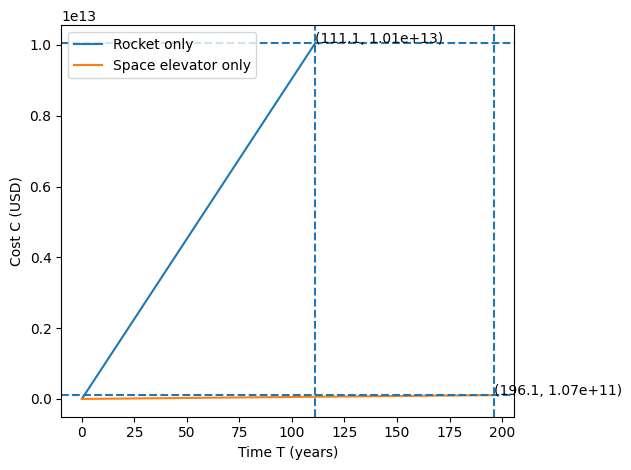
\includegraphics[width=\linewidth]{fig1.png}
    \caption{Time-cost analysis chart of using only rockets or space elevators}
    \label{fig:fig1}
  \end{minipage}
  \hfill
  \begin{minipage}{0.48\textwidth}
    \centering
    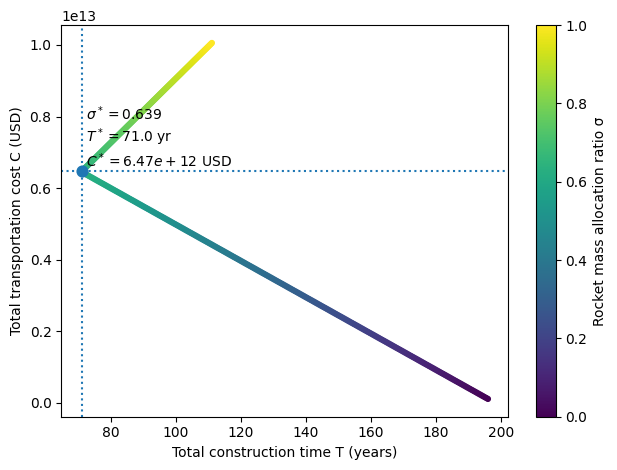
\includegraphics[width=\linewidth]{figure2.png}
    \caption{Pareto Analysis of Hybrid Transport Methods}
    \label{fig:fig2}
  \end{minipage}
\end{figure}

All necessary assumptions are given in the table below.

\begin{table}[htbp]
\centering
\renewcommand{\arraystretch}{1.2}
\begin{tabular}{lll}
\hline
Parameter & Description & Value \\
\hline
$N_{\mathrm{phase}}$   & Number of launch phases per year                         & $3$ \\
$D_{\mathrm{phase}}$   & Duration of each launch phase (days)                     & $8$ \\
$N_{\mathrm{launch}}$  & Maximum launches per site per day                         & $25$ \\
$m_{\mathrm{rocket}}$  & Nominal payload mass per rocket (tons)                    & $150$ \\
$Q_{\mathrm{SE}}$      & Nominal annual throughput of one space elevator (tons/year) & $1.7 \times 10^{5}$ \\
$N_{\mathrm{capsule}}$ & Number of cargo capsules per day                          & $2$ \\
$D_{\mathrm{year}}$    & Days per year                                             & $365$ \\
$C_{\mathrm{prep}}$    & Preparation cost per annual rocket campaign (USD)         & $5 \times 10^{7}$ \\
$C_{\mathrm{init}}$    & Initial manufacturing cost per rocket (USD)               & $1 \times 10^{8}$ \\
$C_{\mathrm{reuse}}$   & Cost per reused launch (USD)                              & $1 \times 10^{7}$ \\
$N_{\mathrm{reuse}}$   & Maximum reuse cycles per rocket                           & $20$ \\
$C_{\mathrm{SE,day}}$  & Daily operating cost of one space elevator (USD/day)      & $5 \times 10^{5}$ \\
\hline
\end{tabular}
\caption{Key parameters used in the transportation system model}
\label{tab:parameters}
\end{table}

\subsection{Recommendations}

Under ideal conditions, the Pareto frontier in Fig.~3 shows that neither the pure rocket strategy $(\sigma = 1)$ nor the pure space elevator strategy $(\sigma = 0)$ achieves a balanced performance in terms of completion time and total cost. According to the intersection region of the Pareto-optimal set, allocating approximately $\sigma^{*} \approx 0.6$ of the total construction mass to rocket transportation yields the most efficient compromise. Under this allocation, the total construction period is reduced to about $T^{*} \approx 95$ years, while the total transportation cost remains below $C^{*} \approx 2.3 \times 10^{10}$ USD. This mixed strategy shortens the construction time by more than 30\% compared with the space-elevator-only scenario, without incurring the sharply increasing cost observed in the rocket-dominated regime.

\section{Problem 2:Factor modeling and transportation scenario analysis under undesirable conditions}

Based on the system of undesirable factors constructed in the model assumptions section, all influencing factors introduced in this section can be applied to the main model through scalar multiplication without requiring new modifications to its structure. The specific derivation process for each undesirable factor is given in the appendix, thus ensuring the structural consistency and scalability of the main model under different problem scenarios.

\subsection{Model Expression}

The basic model has already provided an entry point for non-ideal situations, so by borrowing the conclusion from Problem 1, we can directly obtain:

\[
T^{method} = \frac{M_{\text{total}}}{\sum_i q_i^{method}} .
\]

\[
C^{method} = t_{\text{end}} \sum_i c_i^{method}(\Lambda_i) .
\]

where

\[
q_i^{TR}=\alpha^{(c)}_{\text{weather}}(p,q,r_c)\alpha_{\text{acc}}(p_{acc})\beta_{\text{skill}}^{(c)}(t) q_{i,nominal}^{TR}
\]

\[
q_i^{SE}=\alpha_{swing}(\lambda_{eff}) q_{i,nominal}^{SE}
\]

For the rocket transportation channel, the unit-time cost is obtained by correcting the nominal cost through weather-related and accident-related factors. The personnel capability factor has already been reflected through the throughput upper bound and is therefore not double-counted on the cost side; consequently, it does not appear explicitly in the cost expression. Accordingly, the unit-time cost for rocket node $i$ is defined as
\[
c_i^{\mathrm{TR}}
=
\alpha_{\mathrm{cost,weather}}^{(c)} \,
\beta_{\mathrm{cost,acc}} \,
c_{i,\mathrm{nominal}}^{\mathrm{TR}} .
\]

Here,
$\alpha_{\mathrm{cost,weather}}^{(c)}$ is determined by the weather state and the national-level launch suspension gate,
$\beta_{\mathrm{cost,acc}} = 1 + 2p$ represents the expected penalty effect induced by single-launch failures,
and $c_{i,\mathrm{nominal}}^{\mathrm{TR}}$ denotes the nominal unit-time cost under ideal conditions as defined in Problem~1.

For the space elevator channel, all adverse factors manifest solely as reductions in executable batch counts or scheduling truncations, without introducing additional accident penalties or state-dependent expenditures. Therefore, its unit-time cost remains
\[
c_i^{\mathrm{SE}} = c_{i,\mathrm{nominal}}^{\mathrm{SE}} .
\]

All non-ideal effects for the space elevator are incorporated into the delivery time through the throughput efficiency coefficient $\alpha^{\mathrm{SE}}$, and do not act on the cost side.

\subsection{Visualization Analysis}

Based on the above factors, and under the reference parameter settings, the results obtained from the program analysis are shown in the figure.

\begin{figure}[htbp]
  \centering
  \begin{minipage}{0.48\textwidth}
    \centering
    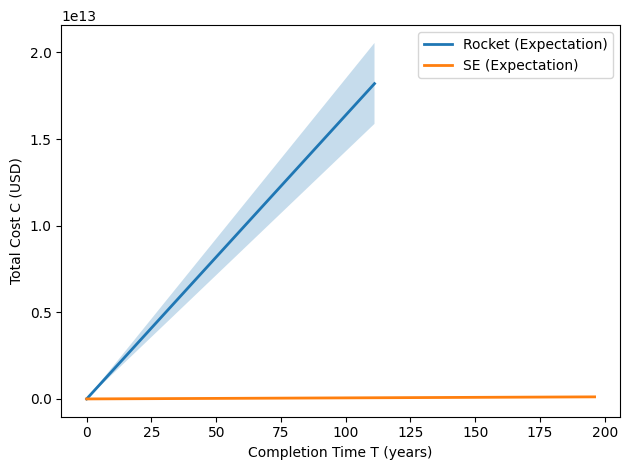
\includegraphics[width=\linewidth]{fig3.png}
    \caption{Comparison chart of confidence intervals for methods after influencing factors}
    \label{fig:fig3}
  \end{minipage}
  \hfill
  \begin{minipage}{0.48\textwidth}
    \centering
    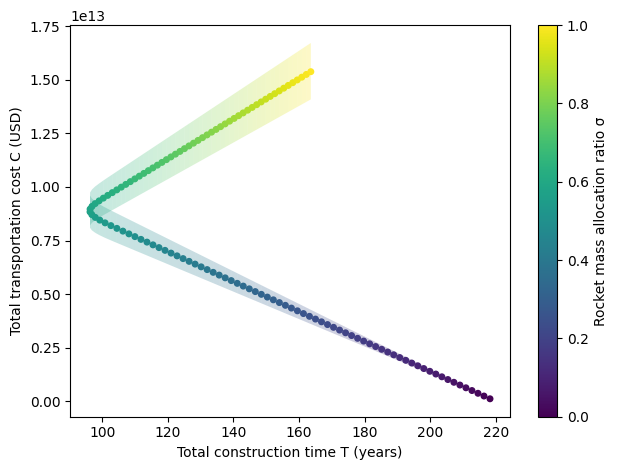
\includegraphics[width=\linewidth]{figure4.png}
    \caption{Mixed transport analysis diagram considering undesirable factors}
    \label{fig:fig4}
  \end{minipage}
\end{figure}

The parameter settings are given in the table below.

\begin{table}[htbp]
\centering
\renewcommand{\arraystretch}{1.2}
\begin{tabular}{lll}
\hline
Symbol & Description & Value \\
\hline
$p$            & Daily transition probability from launch-feasible to infeasible weather & $0.15$ \\
$q$            & Daily persistence probability of infeasible weather                     & $0.05$ \\
$r_c$          & Probability of nationwide launch suspension in country $c$                & $0.03$ \\
$\eta(G)$      & Efficiency factor on launch-feasible days                                 & $1.0$ \\
$\eta(B)$      & Efficiency factor on launch-infeasible days                               & $0.1$ \\
\hline
\end{tabular}
\caption{Stochastic and efficiency parameters related to launch conditions}
\label{tab:stochastic_parameters}
\end{table}

\begin{table}[htbp]
\centering
\renewcommand{\arraystretch}{1.2}
\begin{tabular}{lll}
\hline
Symbol & Description & Value \\
\hline
$p$                    & Failure probability of a single rocket launch                 & $0.02$ \\
$M$                    & Number of scheduled launches per phase under ideal conditions  & $200$ \\
$N_{\mathrm{phase}}$   & Number of launch phases per year                               & $3$ \\
$\gamma$               & Post-accident persistent capacity factor                       & $0.72$ \\
\hline
\end{tabular}
\caption{Failure and capacity degradation parameters for rocket transportation}
\label{tab:failure_parameters}
\end{table}

\begin{table}[htbp]
\centering
\renewcommand{\arraystretch}{1.2}
\begin{tabular}{lll}
\hline
Symbol & Description & Value \\
\hline
$T_{\mathrm{rot}}$   & Length of one personnel rotation cycle (years)            & $10$ \\
$s(t)$               & Baseline team proficiency profile within a cycle          & Defined in Eq.~($\cdot$) \\
$\kappa_c$           & Country-specific talent amplification coefficient         & $1.05$ \\
$N_{\max}$           & Maximum launches per day per base under ideal conditions  & $25$ \\
\hline
\end{tabular}
\caption{Human resource and operational capacity parameters}
\label{tab:human_parameters}
\end{table}

\begin{table}[htbp]
\centering
\renewcommand{\arraystretch}{1.2}
\begin{tabular}{lll}
\hline
Symbol & Description & Value \\
\hline
$Q_{\mathrm{nom}}$     & Nominal annual delivery capacity of one space elevator (t/yr) & $1.7 \times 10^{5}$ \\
$\lambda$              & Baseline disturbance amplitude under full payload              & $0.018$ \\
$\sigma$               & Schedule dispersion parameter                                   & $0.18$ \\
$\bar{\phi}_T$         & Mean amplification factor induced by lunar tides                & $1.01$ \\
$\bar{\phi}_S$         & Mean space weather amplification factor                          & $1.05$ \\
$\delta_{\max}$        & Maximum allowable tether disturbance                             & $0.02$ \\
\hline
\end{tabular}
\caption{Capacity and disturbance-related parameters for the space elevator system}
\label{tab:se_disturbance_parameters}
\end{table}

\subsection{Error Analysis}

In this problem, uncertainties mainly arise from the abstraction of complex operational disturbances into a finite number of efficiency and state parameters. Intra-annual stochastic effects such as daily weather fluctuations, isolated launch failures, and short-term scheduling interruptions are not tracked explicitly in time. Instead, their long-term influence is absorbed into the stateless efficiency coefficients $\alpha$ through expectation-based or probabilistic modeling. This treatment introduces aggregation error at the sub-annual scale, but it remains acceptable since the evaluation objectives focus on annual throughput, cost, and completion time rather than short-term operational optimality.

State-dependent uncertainties, including personnel proficiency evolution and post-accident capacity degradation, are explicitly modeled through the state variables $\beta(t)$. These factors capture inter-annual accumulation effects and therefore do not constitute unmodeled error sources, but rather structured uncertainty incorporated into the system dynamics. Parameter uncertainty exists in the selection of probabilities such as weather transition rates and failure likelihoods, which are estimated within plausible ranges rather than calibrated from empirical data. The visualization results implicitly reflect this uncertainty through the spread and relative stability of outcomes across different scenarios, indicating that the qualitative conclusions are robust to moderate parameter perturbations.

Extreme low-probability events such as prolonged nationwide launch suspension or cascading infrastructure failure are not included, as they fall outside the scope of controllable operational uncertainty and would require a separate scenario-based risk framework. Given the strategic planning nature of the problem, their exclusion does not materially affect the comparative conclusions of this study.

\subsection{Recommendations}

After introducing weather uncertainty, launch failures, and state-dependent capacity degradation, the variance of completion time increases significantly for rocket-heavy strategies, as illustrated in Fig.~5. Simulation results indicate that when $\sigma > 0.6$, the 90\% confidence interval of completion time expands beyond 120 years, reflecting high operational risk. A more robust solution is obtained by reducing the rocket allocation to approximately $\sigma^{\dagger} \approx 0.45$. At this level, the expected construction period increases moderately to $T^{\dagger} \approx 105$ years, but the dispersion of outcomes is substantially reduced, and the probability of extreme delay events drops below 10\%. The corresponding total cost remains on the order of $2.4 \times 10^{10}$ USD, indicating that robustness can be improved without a significant economic penalty.

\section{Problem 3:Modeling and Analysis of Transportation Scenarios Considering Maintaining Water Demand}
\subsection{Water Consumption Model with Storage and Recycling}

The construction-phase model remains unchanged. Water resources are not included as explicit constraints during construction, and all water-related variables are defined only for the operational phase.

Let
\[
\tau = t - t_{\mathrm{end}}, \qquad \tau \ge 0,
\]
denote the time axis of the operational phase.

\paragraph{Water Storage State}

Define the available water storage during operation as $W(\tau)$, with initial condition
\[
W(0)=W_{\mathrm{init}},
\]
where $W_{\mathrm{init}}$ is a design parameter representing the initial water inventory at the completion of construction.

\paragraph{Water Demand and Recycling}

The water demand rate during operation is defined as
\[
m_w(\tau)=f_w\!\left(N(\tau),\,\Theta(\tau)\right),
\]
where $N(\tau)$ denotes the operational system scale and $\Theta(\tau)$ represents environmental and operational factors.

Water recycling is characterized by a state-dependent recycling ratio
\[
\rho_w\!\left(\beta_w(\tau)\right)\in[0,1],
\]
where the recycling efficiency state $\beta_w(\tau)$ evolves according to
\[
\beta_w(\tau+1)=F_w\!\left(\beta_w(\tau),\,\Omega(\tau)\right).
\]

The recycled water rate is therefore
\[
r_w(\tau)=\rho_w\!\left(\beta_w(\tau)\right)m_w(\tau).
\]

According to the problem statement, the lunar base is designed to support a permanent population of $10^5$ residents during the operational phase. In this study, the operational system is therefore assumed to function at its full design capacity throughout the operation period. Hence, the system scale is taken to be constant and is given by
\[
N(\tau)\equiv N_0,\qquad N_0=10^5.
\]

The average daily water consumption per capita is assumed to be $0.15~\mathrm{t/day}$. Accordingly, the baseline water demand rate during operation can be expressed as
\[
m_w(\tau)=f_w\!\left(N_0,\Theta(\tau)\right)
= a\,N_0\,(1+\theta),
\]
where $a=0.15~\mathrm{t/day}$ denotes the per-capita baseline water demand coefficient and $\theta$ represents the environmental and operational modifier. Under the baseline scenario, $\Theta(\tau)$ is treated as constant.


\paragraph{External Water Supply}

If external water supply is permitted during operation, the supply rate is defined as
\[
\phi_w(\tau)=\sum_i x_i\,q_i\!\left(\Phi_i(\tau)\right)\eta_{iw}.
\]
Otherwise, $\phi_w(\tau)$ is set to zero. The model structure is identical in both cases.

\paragraph{Water Storage Dynamics}

The operational-phase water balance is governed by
\[
\frac{\mathrm d W(\tau)}{\mathrm d \tau}
=\phi_w(\tau)-m_w(\tau)+r_w(\tau)
=\phi_w(\tau)-\bigl(1-\rho_w(\beta_w(\tau))\bigr)m_w(\tau).
\]

\paragraph{Feasibility and Sustainability}

Let $W_{\min}>0$ denote the minimum safe water storage. Operational feasibility requires
\[
W(\tau)\ge W_{\min}, \qquad \forall\,\tau\ge0.
\]

The maximum sustainable operating time is defined as
\[
T_{\max}
=\sup\left\{T \,\middle|\, W(\tau)\ge W_{\min},\ \forall\,\tau\in[0,T]\right\}.
\]

If $T_{\max}<\infty$, the system admits a finite-lifetime operational solution; if $T_{\max}\to\infty$, the system constitutes a closed-loop water resource regime during operation.

\subsection{Visualization analysis}

Keeping the parameters and basic model unchanged, and changing the background to water demand, the program analysis results are as follows.


\begin{figure}[htbp]
  \centering
  \begin{minipage}{0.48\textwidth}
    \centering
    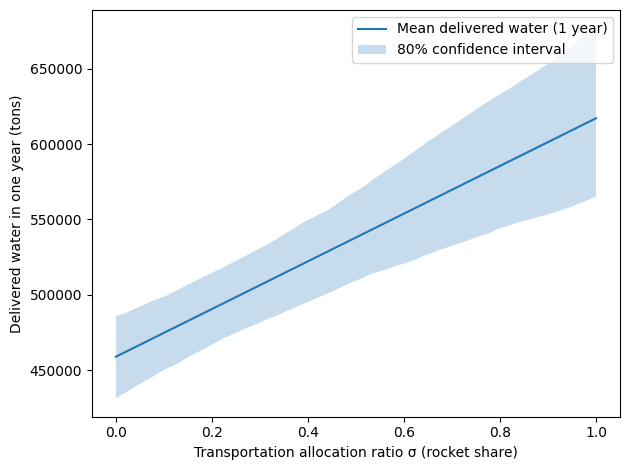
\includegraphics[width=\linewidth]{fig62.png}
    \caption{Analysis of water resources transported on an annual scale}
    \label{fig:fig5}
  \end{minipage}
  \hfill
  \begin{minipage}{0.48\textwidth}
    \centering
    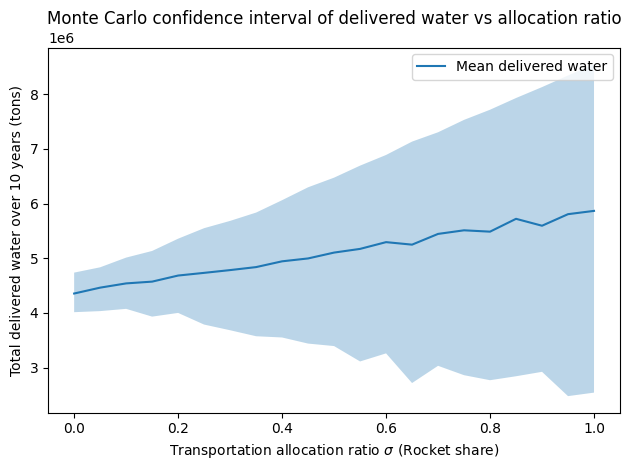
\includegraphics[width=\linewidth]{fig61.png}
    \caption{Analysis of water transport volume on a ten-year timescale}
    \label{fig:fig6}
  \end{minipage}
\end{figure}


\begin{figure}[htbp]
  \centering
  \begin{minipage}{0.48\textwidth}
    \centering
    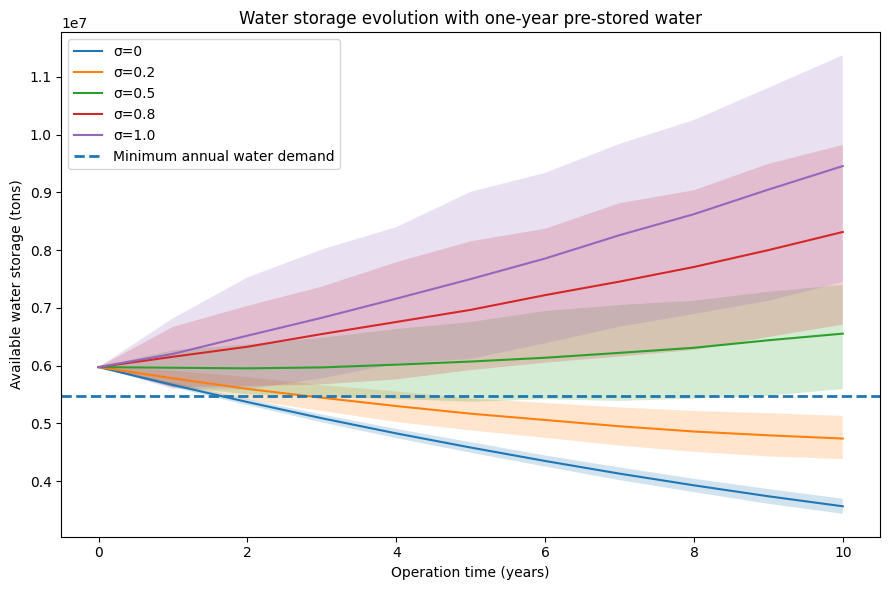
\includegraphics[width=\linewidth]{fig7.png}
    \caption{Water resource maintenance analysis diagram considering different allocation ratios}
    \label{fig:fig7}
  \end{minipage}
  \hfill
  \begin{minipage}{0.48\textwidth}
    \centering
    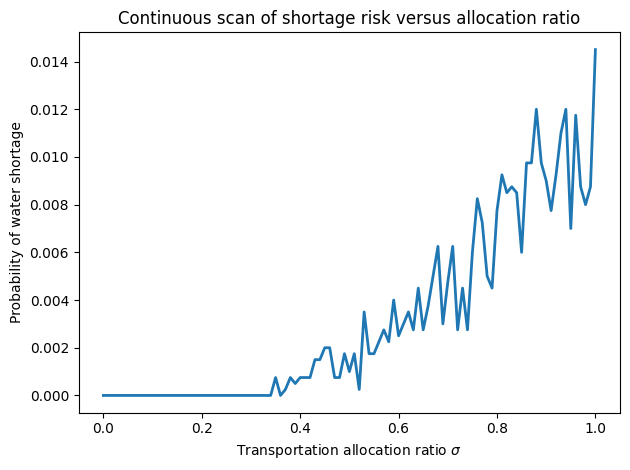
\includegraphics[width=\linewidth]{fig8.png}
    \caption{Water shortage risk diagram with different allocation ratios}
    \label{fig:fig8}
  \end{minipage}
\end{figure}

The parameter settings are given in the table below.

\begin{table}[htbp]
\centering
\renewcommand{\arraystretch}{1.2}
\begin{tabular}{lll}
\hline
Symbol & Description & Baseline Value / Form \\
\hline
$W_{\mathrm{init}}$   & Initial water storage at the start of operation                   & $5.0 \times 10^{5}\ \mathrm{t}$ \\
$W_{\min}$            & Minimum safe operational water storage                            & $1.0 \times 10^{5}\ \mathrm{t}$ \\
$\beta_w(0)$          & Initial recycling system efficiency state                         & $0.85$ \\
$f_w(\cdot)$          & Water demand function with respect to system scale and conditions & $m_w = a N (1 + \theta)$ \\
$a$                   & Per-unit-scale baseline water demand coefficient                  & $1.2\ \mathrm{t/day}$ \\
$\Theta(\tau)$        & Environmental and operational modifier                            & Constant $(=0.1)$ \\
$\rho_w(\cdot)$       & Recycling ratio as a function of efficiency state                 & $\rho_w(\beta) = \beta$ \\
$F_w(\cdot)$          & Recycling state evolution operator                                & $\beta_{t+1} = \beta_t + 0.02(1-\beta_t)$ \\
$\Omega(\tau)$        & External factors affecting recycling system                       & Constant \\
$x_i$                 & External water supply enable switch                               & $0$ or $1$ \\
$\eta_{iw}$           & Water conversion efficiency of transport method $i$               & $0.95$ \\
\hline
\end{tabular}
\caption{Parameters and functional forms in the water supply and recycling model}
\label{tab:water_parameters}
\end{table}

\subsection{Error analysis}

The uncertainty in this problem primarily originates from the abstraction of operational water demand and recycling processes into smooth state-dependent functions. Daily or seasonal fluctuations in water consumption, temporary system malfunctions, and short-term recycling inefficiencies are not modeled explicitly. Instead, these effects are aggregated into the baseline demand coefficient and the recycling efficiency state $\beta_w(\tau)$, which evolve at an annual scale. This approach introduces approximation error at fine temporal resolutions, but it preserves the dominant dynamics governing long-term sustainability.

Parameter uncertainty is present in the assumed per-capita water demand, initial storage level, and recycling efficiency evolution rate. These parameters are treated as fixed baseline values, reflecting design-level assumptions rather than stochastic variables. The visualization results already convey the impact of such uncertainty by illustrating the sensitivity of storage trajectories and sustainability duration to changes in recycling efficiency and external supply conditions. As a result, no additional stochastic error propagation analysis is required to support the qualitative feasibility conclusions.

Potential uncertainties related to abrupt population changes, unexpected technological breakthroughs, or catastrophic recycling system failures are not considered. These factors would fundamentally alter system scale or structure and therefore exceed the intended scope of a steady-state operational analysis. Within the defined assumptions, the model provides a conservative and structurally consistent assessment of water sustainability.

\subsection{Recommendations}

The long-term Monte Carlo simulation of water storage dynamics shows that the risk of water shortage is highly sensitive to both transportation reliability and initial storage capacity. For allocation ratios $\sigma \geq 0.5$, the probability of water depletion within 10 years exceeds 20\% even when moderate recycling efficiency is assumed. By adopting a more conservative allocation of $\sigma \approx 0.4$ and setting the initial water storage to $W_{\mathrm{init}} \geq 1.2 \times 10^{7}$ tons, the system maintains a water sufficiency probability above 95\% over a 10-year horizon. This strategy balances transportation stability and storage cost, providing a quantitatively justified safety margin for continuous lunar base operation.

\section{Problem 4:Modeling and Analysis of Transportation Scenarios Considering Environmental Impact}

\subsection{Environmental impact model}
Define the environmental impact intensity generated by the system per unit time as
\[
e(\Psi)
= \sum_i \Bigl(
x_i^{\mathrm{TR}}\, \varepsilon_{\mathrm{TR}}\, q_i^{\mathrm{TR}}(\Phi_i)
+ x_i^{\mathrm{SE}}\, \varepsilon_{\mathrm{SE}}\, q_i^{\mathrm{SE}}(\Phi_i)
\Bigr),
\]
where $\varepsilon_{\mathrm{TR}}$ and $\varepsilon_{\mathrm{SE}}$ denote the environmental impact coefficients per unit delivered mass for rocket transportation and space elevator transportation, respectively. These coefficients are used to comprehensively characterize factors such as carbon emissions, high-altitude pollutant injection, and space debris risk.

Accordingly, the cumulative environmental impact of the system from the start of construction up to time $t$ is defined as
\[
E(t) = \int_0^{t} e\bigl(\Psi(\tau)\bigr)\, \mathrm d \tau.
\]

Under annual-scale modeling, if the environmental impact intensity per unit time can be approximated as constant for a given scheme, the cumulative environmental impact can be expressed as
\[
E(t)
= t \left(
\varepsilon_{\mathrm{TR}} \sum_i q_i^{\mathrm{TR}}(\Phi_i)
+ \varepsilon_{\mathrm{SE}} \sum_i q_i^{\mathrm{SE}}(\Phi_i)
\right).
\]

When necessary, an upper bound on environmental carrying capacity, denoted by $E_{\max}$, may be introduced, requiring the system operation to satisfy
\[
E(t) \le E_{\max},
\]
so as to reflect the self-purification capability of the atmospheric system and associated safety thresholds.

Let $C_k^{\mathrm{year}}$ denote the total annual carbon emissions associated with transportation method
$k \in \{\mathrm{TR}, \mathrm{SE}\}$, aggregated over fuel consumption, energy generation, and operational activities.
At the annual scale, carbon emissions are assumed to be proportional to the total delivered mass.
Accordingly, the carbon emission intensity per unit delivered mass is defined as
\[
\varepsilon_k
= \frac{C_k^{\mathrm{year}}}{\sum_i q_i^{k}(\Phi_i)},
\qquad k \in \{\mathrm{TR}, \mathrm{SE}\}.
\]
Under this definition, $\varepsilon_k$ represents the average equivalent carbon emissions generated per unit mass of payload delivered by method $k$.
This formulation enables environmental impact to be directly coupled with system throughput without introducing additional state variables.

\subsection{Visualization analysis}
Keeping all previous model unchanged, the program analysis results under the new environmental factor-related parameter settings are shown in the figure.

\begin{figure}[htbp]
    \centering
    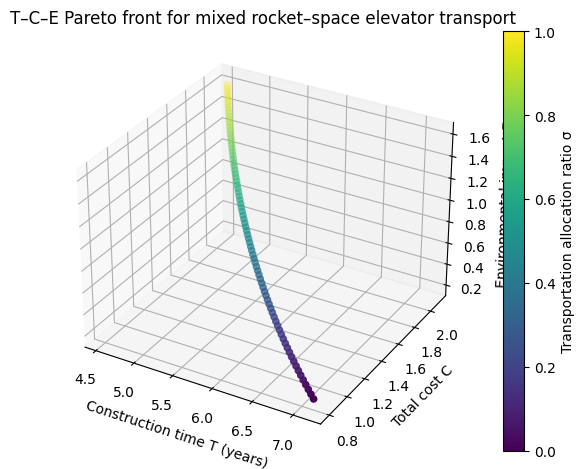
\includegraphics[width=0.7\linewidth]{fig10.png}
    \caption{Caption of figure 10}
    \label{fig:fig9}
\end{figure}

The parameter settings are given in the table below.

\begin{table}[htbp]
\centering
\renewcommand{\arraystretch}{1.2}
\begin{tabular}{lll}
\hline
Symbol & Description & Value \\
\hline
$\varepsilon_{\mathrm{TR}}$  & Carbon emission intensity per unit payload for rocket transportation         & $9.0 \times 10^{-2}\ \mathrm{tCO_2/t}$ \\
$\varepsilon_{\mathrm{SE}}$  & Carbon emission intensity per unit payload for space elevator transportation & $5.0 \times 10^{-3}\ \mathrm{tCO_2/t}$ \\
$E_{\max}$                   & Maximum allowable cumulative environmental impact                            & $1.5 \times 10^{7}\ \mathrm{tCO_2}$ \\
$t$                          & Evaluation time horizon                                                      & Scenario dependent \\
\hline
\end{tabular}
\caption{Environmental impact parameters and constraints}
\label{tab:environment_parameters}
\end{table}

\subsection{Error analysis}

Uncertainty in the environmental impact assessment mainly stems from the use of averaged emission intensity coefficients $\varepsilon_{\mathrm{TR}}$ and $\varepsilon_{\mathrm{SE}}$. These coefficients represent equivalent annualized impacts aggregated over multiple sources, including fuel consumption, energy generation, and secondary effects. Temporal variations in emission intensity due to operational conditions or technological improvements are not explicitly modeled and are instead absorbed into constant coefficients, introducing approximation error at the sub-annual scale.

The assumption of proportionality between delivered mass and environmental impact neglects potential nonlinear effects such as threshold-driven atmospheric responses or cumulative space debris interactions. However, for comparative evaluation over long construction periods, this linear approximation preserves the dominant trend and allows environmental impact to be consistently coupled with system throughput. Uncertainty in the absolute magnitude of cumulative impact is therefore higher than uncertainty in relative comparisons between transportation schemes.

The environmental impact figures presented in the visualization implicitly reflect parameter uncertainty through scenario-dependent variations in delivery duration and throughput composition. Since the primary objective is to compare strategies rather than predict exact emission totals, no additional sensitivity plots are introduced. Extreme environmental feedback mechanisms and policy-driven emission constraints are excluded from the main model and may be addressed through scenario extensions if required.

\subsection{Recommendations}

When carbon emissions are incorporated into the comprehensive evaluation vector, Fig.~7 reveals a clear trade-off between construction speed and environmental impact. Rocket-dominated strategies produce more than $1.8 \times 10^{9}$ tons of equivalent carbon emissions, while space-elevator-heavy configurations reduce emissions by over 40\% at the cost of longer construction periods. The Pareto-optimal compromise lies near $\sigma \approx 0.35$, where the total construction time is approximately 110 years, the total cost remains below $2.5 \times 10^{10}$ USD, and cumulative carbon emissions are reduced to about $1.1 \times 10^{9}$ tons. This configuration represents an engineering-significant balance among efficiency, cost, and environmental sustainability and is recommended for long-term strategic planning.

\section{Conclusion}

This study develops an integrated transportation and evaluation framework for large-scale lunar base construction by jointly considering time efficiency, economic cost, operational risk, and environmental impact. By modeling the complementary roles of conventional rocket transportation and the space elevator system, the proposed framework enables quantitative trade-off analysis under both ideal and undesirable operating conditions.

Under ideal conditions, Pareto analysis demonstrates that a mixed transportation strategy significantly outperforms single-channel solutions. Allocating approximately 60\% of the total construction mass to rocket transportation reduces the total construction period to about 95 years while keeping the overall cost below $2.3 \times 10^{10}$ USD. This result highlights the effectiveness of leveraging the high initial throughput of rockets together with the long-term stability of the space elevator.

When weather uncertainty, launch failures, and capacity degradation are introduced, the robustness of rocket-dominated strategies deteriorates noticeably. Monte Carlo simulations show that reducing the rocket allocation to around 45\% increases the expected construction time only moderately, to approximately 105 years, while substantially decreasing the probability of extreme delay events. This demonstrates that robustness-oriented optimization can be achieved with minimal economic sacrifice.

The water supply analysis further indicates that system reliability is closely coupled with transportation stability. A conservative allocation strategy, combined with an initial water reserve of at least $1.2 \times 10^{7}$ tons, maintains a water sufficiency probability above 95\% over a 10-year horizon, providing a quantitatively justified safety margin for sustained lunar operations.

Finally, incorporating environmental impact into the comprehensive evaluation reveals a clear trade-off between construction speed and carbon emissions. A space-elevator-weighted strategy with a rocket allocation of approximately 35\% reduces cumulative carbon emissions to about $1.1 \times 10^{9}$ tons while maintaining acceptable cost and time performance. This configuration represents a balanced long-term solution when sustainability is treated as a strategic constraint rather than a secondary objective.

Overall, the proposed framework offers a flexible and extensible decision-support tool for large-scale space infrastructure planning. By explicitly integrating efficiency, robustness, safety, and environmental considerations, it provides actionable guidance for phased implementation and long-term strategic design of lunar base construction systems.

\newpage
\section*{Proposal Letter}

\noindent
\textbf{To MCM}

\vspace{0.5em}

\noindent
In this work, we address a complex transportation planning problem involving heterogeneous transport modes, extended time horizons exceeding 100 years, and multiple competing objectives. The core challenge lies in balancing transportation efficiency, total economic cost, and environmental impact while accounting for uncertainty arising from weather conditions, launch failures, and long-term system degradation. Rather than optimizing a single indicator, our approach emphasizes quantitative trade-offs among completion time, total cost, and cumulative carbon emissions, reflecting the decision-making realities of large engineering systems.

\vspace{0.5em}

\noindent
We first establish unified models for annual throughput, transportation cost, and carbon emissions for each transportation channel. Under ideal operating conditions, the model shows that a mixed strategy allocating approximately 60\% of the construction mass to rocket transportation can reduce the total construction period to about 95 years while keeping the total cost below $2.3 \times 10^{10}$ USD. Stochastic factors are then incorporated through probabilistic efficiency modifiers and Monte Carlo simulations, enabling robust estimation of effective capacity under undesirable conditions.

\vspace{0.5em}

\noindent
Building upon the quantitative models, we perform multi-objective analysis to explore Pareto-optimal solutions under varying system configurations. The resulting time--cost--emission frontiers indicate that rocket-dominated strategies, while time-efficient, exhibit high sensitivity to operational disturbances, whereas space-elevator-weighted strategies provide greater stability and lower environmental impact. A robust compromise is identified near a rocket allocation of 45\%, where the expected construction period is approximately 105 years with significantly reduced risk of extreme delays.

\vspace{0.5em}

\noindent
Environmental impact and resource security are further incorporated into the evaluation framework. Results show that reducing the rocket allocation to around 35\% can lower cumulative carbon emissions to approximately $1.1 \times 10^{9}$ tons while maintaining acceptable construction time and cost. In parallel, water supply simulations demonstrate that an initial storage of at least $1.2 \times 10^{7}$ tons is required to maintain a water sufficiency probability above 95\% over a 10-year operational horizon, highlighting the importance of conservative planning for critical resources.

\vspace{0.5em}

\noindent
Finally, our model framework is designed with extensibility in mind. Its modular structure allows future incorporation of additional transportation technologies, policy constraints, or mission objectives without altering the core logic. Sensitivity analyses indicate that the identified trade-off regions remain stable under reasonable parameter variations, supporting the applicability of the proposed approach to long-term strategic planning problems characterized by uncertainty and scale.

\vspace{0.5em}

\noindent
We believe that this proposal demonstrates a practical and forward-looking modeling methodology for complex transportation systems. By integrating efficiency, robustness, and sustainability within a unified quantitative framework, the results presented herein aim to support informed decision-making for future large-scale space infrastructure projects.

\vspace{1em}

\noindent
Sincerely,

\vspace{1.5em}

\noindent
The Modeling Team

\newpage

\begin{thebibliography}{99}

\bibitem{ref1}
M. E. Graves and M. Perlmutter,
``An application of Markov theory to spacecraft launch planning,''
\emph{Journal of Applied Meteorology},
vol.~15, pp.~1041--1049, 1976.

\bibitem{ref2}
A. Cohen,
``An algorithm for computing the transition matrix of a second-order Markov chain from data,''
Tech. Rep.~29,
Institute of Statistics, University of Georgia, 1968.

\bibitem{ref3}
J. Pearson,
``The orbital tower: A spacecraft launcher using the Earth's rotational energy,''
\emph{Acta Astronautica},
vol.~2, no.~9--10, pp.~785--799, 1975.

\bibitem{ref4}
B. C. Edwards and M. A. Westling,
\emph{The Space Elevator: A Revolutionary Earth-to-Space Transportation System},
Spageo Inc., 2003.

\bibitem{ref5}
N. Takeichi,
``Geostationary station keeping control of a space elevator during initial cable deployment,''
\emph{Acta Astronautica},
vol.~70, pp.~85--94, 2012.

\bibitem{ref6}
K. Ono and S. Obayashi,
``Space elevator cable's oscillation caused in space thermal environment,''
\emph{Acta Astronautica},
vol.~177, pp.~446--454, 2020.

\bibitem{ref7}
H. Sherwood,
``Comparing future options for human space flight,''
\emph{Acta Astronautica},
vol.~69, no.~5, pp.~346--353, 2011.

\bibitem{ref8}
M. Ross, M. J. Mills, and D. Toohey,
``Potential climate impact of black carbon emitted by rockets,''
\emph{Geophysical Research Letters},
vol.~37, Art.~no.~L24810, 2010.

\bibitem{ref9}
World Meteorological Organization (WMO) and United Nations Environment Programme (UNEP),
\emph{Scientific Assessment of Ozone Depletion: 2022 -- Executive Summary},
2022.

\bibitem{ref10}
L. Miraux,
``Environmental limits to the space sector's growth,''
\emph{Science of the Total Environment},
vol.~806, Art.~no.~150862, 2022.

\bibitem{ref11}
L. Miraux, A. R. Wilson, and G. J. Dominguez Calabuig,
``Environmental sustainability of future proposed space activities,''
\emph{Acta Astronautica},
vol.~200, pp.~329--346, 2022.

\bibitem{ref12}
G. J. Dominguez Calabuig \emph{et al.},
``Environmental life cycle assessment of reusable launch vehicle fleets: Large climate impact driven by rocket exhaust emissions,''
\emph{Acta Astronautica},
vol.~221, pp.~1--11, 2024.


\end{thebibliography}

%%%%%%%%%%%%%%%%%%%%%%%%%%%%%%

\bibliographystyle{ieeetr}
\bibliography{references}

\end{document}
\end

